% ============================================================================
% Capitulo: Resultados y Analisis de la KHI en RRMHD  (orden invertido)
% ----------------------------------------------------------------------------
% CAMBIOS RESPECTO A LA VERSION ANTERIOR:
%   - Titulo del capitulo invertido: "Resultados y Analisis".
%   - NUEVA Seccion 1: Vision global del barrido (ultrawides + tabla canonica).
%   - Figura fig_derivadas_M1_M2.pdf regenerada con dominios independientes
%     en cada panel: la grafica roja (Metodo 2) ahora muestra correctamente
%     las dos jorobas en su dominio de datos [2800, 10500].
%   - Las secciones analiticas restantes (2-7) conservan su estructura.
%
% RESTRICCIONES OBSERVADAS (sin cambios):
%   - No se hace mencion al Numero de Reynolds magnetico Rm.
%   - No se utiliza el criterio de fraccion (f * gamma_0).
%   - No se incluyen las derivadas logaritmicas del t_peak.
%
% Comandos personales asumidos (declarar en el preambulo si no existen):
%   \newcommand{\gKHI}{\gamma_{\mathrm{KHI}}}
%   \newcommand{\Ozp}{\Omega_{zp}}
%   \newcommand{\Omaxzp}{\Omega_{zp}^{\max}}
%   \newcommand{\Otot}{\Omega_{\mathrm{tot}}}
%   \newcommand{\scrit}{\sigma_{\mathrm{crit}}}
%   \newcommand{\akh}{a_{kh}}
%   \newcommand{\leff}{\ell_{\mathrm{eff}}}
%
% Paquetes requeridos para la tabla canonica:
%   \usepackage{longtable}   % O usar tabular convencional en 4 columnas.
% ============================================================================


\primerparrafo Este capítulo presenta el análisis cuantitativo de las simulaciones RRMHD del barrido paramétrico en la conductividad eléctrica $\sigma$, descrito en el Capítulo~\ref{sec:setup_experimental}. La exposición sigue un orden lógico que parte de la fenomenología cruda de las simulaciones (evolución temporal de los diagnósticos globales) y converge hacia los resultados paramétricos derivados: (i) una visualización global del barrido completo de 44 simulaciones a través de las trayectorias temporales de la enstrofía; (ii) un ajuste paramétrico tipo sigmoide que captura la transición continua entre los regímenes resistivo e ideal y permite identificar la tasa de crecimiento asintótica $\gKHI(\sigma\to\infty) \equiv \gamma_0$; (iii) el análisis de las derivadas logarítmicas de los observables principales para estimar la conductividad crítica $\scrit$ y delimitar de manera objetiva las zonas fenomenológicas del flujo; (iv) el estudio de la curva directa $t_{\mathrm{peak}}(\sigma)$ como métrica auxiliar libre de manipulación derivativa; y (v) la confrontación de los exponentes empíricos de la ley de potencias $\Omaxzp(\sigma)$ con las predicciones de la teoría lineal y el análisis de la escala disipativa efectiva del sistema.

\section{Visión global del barrido paramétrico}
\label{sec:vision_global}

\primerparrafo Antes de cualquier análisis derivativo, es indispensable verificar que las 44 simulaciones del barrido reproducen la fenomenología esperada de la KHI en el régimen RRMHD y que las trayectorias temporales de los diagnósticos globales presentan la estructura de tres fases bien delimitadas: (i) fase lineal de crecimiento exponencial, (ii) fase de transición no lineal con formación de vórtices coherentes, y (iii) fase de saturación con eventual disipación residual. Esta verificación se realiza sobre la enstrofía absoluta total $\Otot(t)$ y sobre la enstrofía de perturbación $\Ozp(t)$, observables complementarios cuya construcción se detalló en la Sección~\ref{subsec:diagnostico}.

\subsection{Trayectorias temporales del barrido}

\begin{figure}[H]
\centering
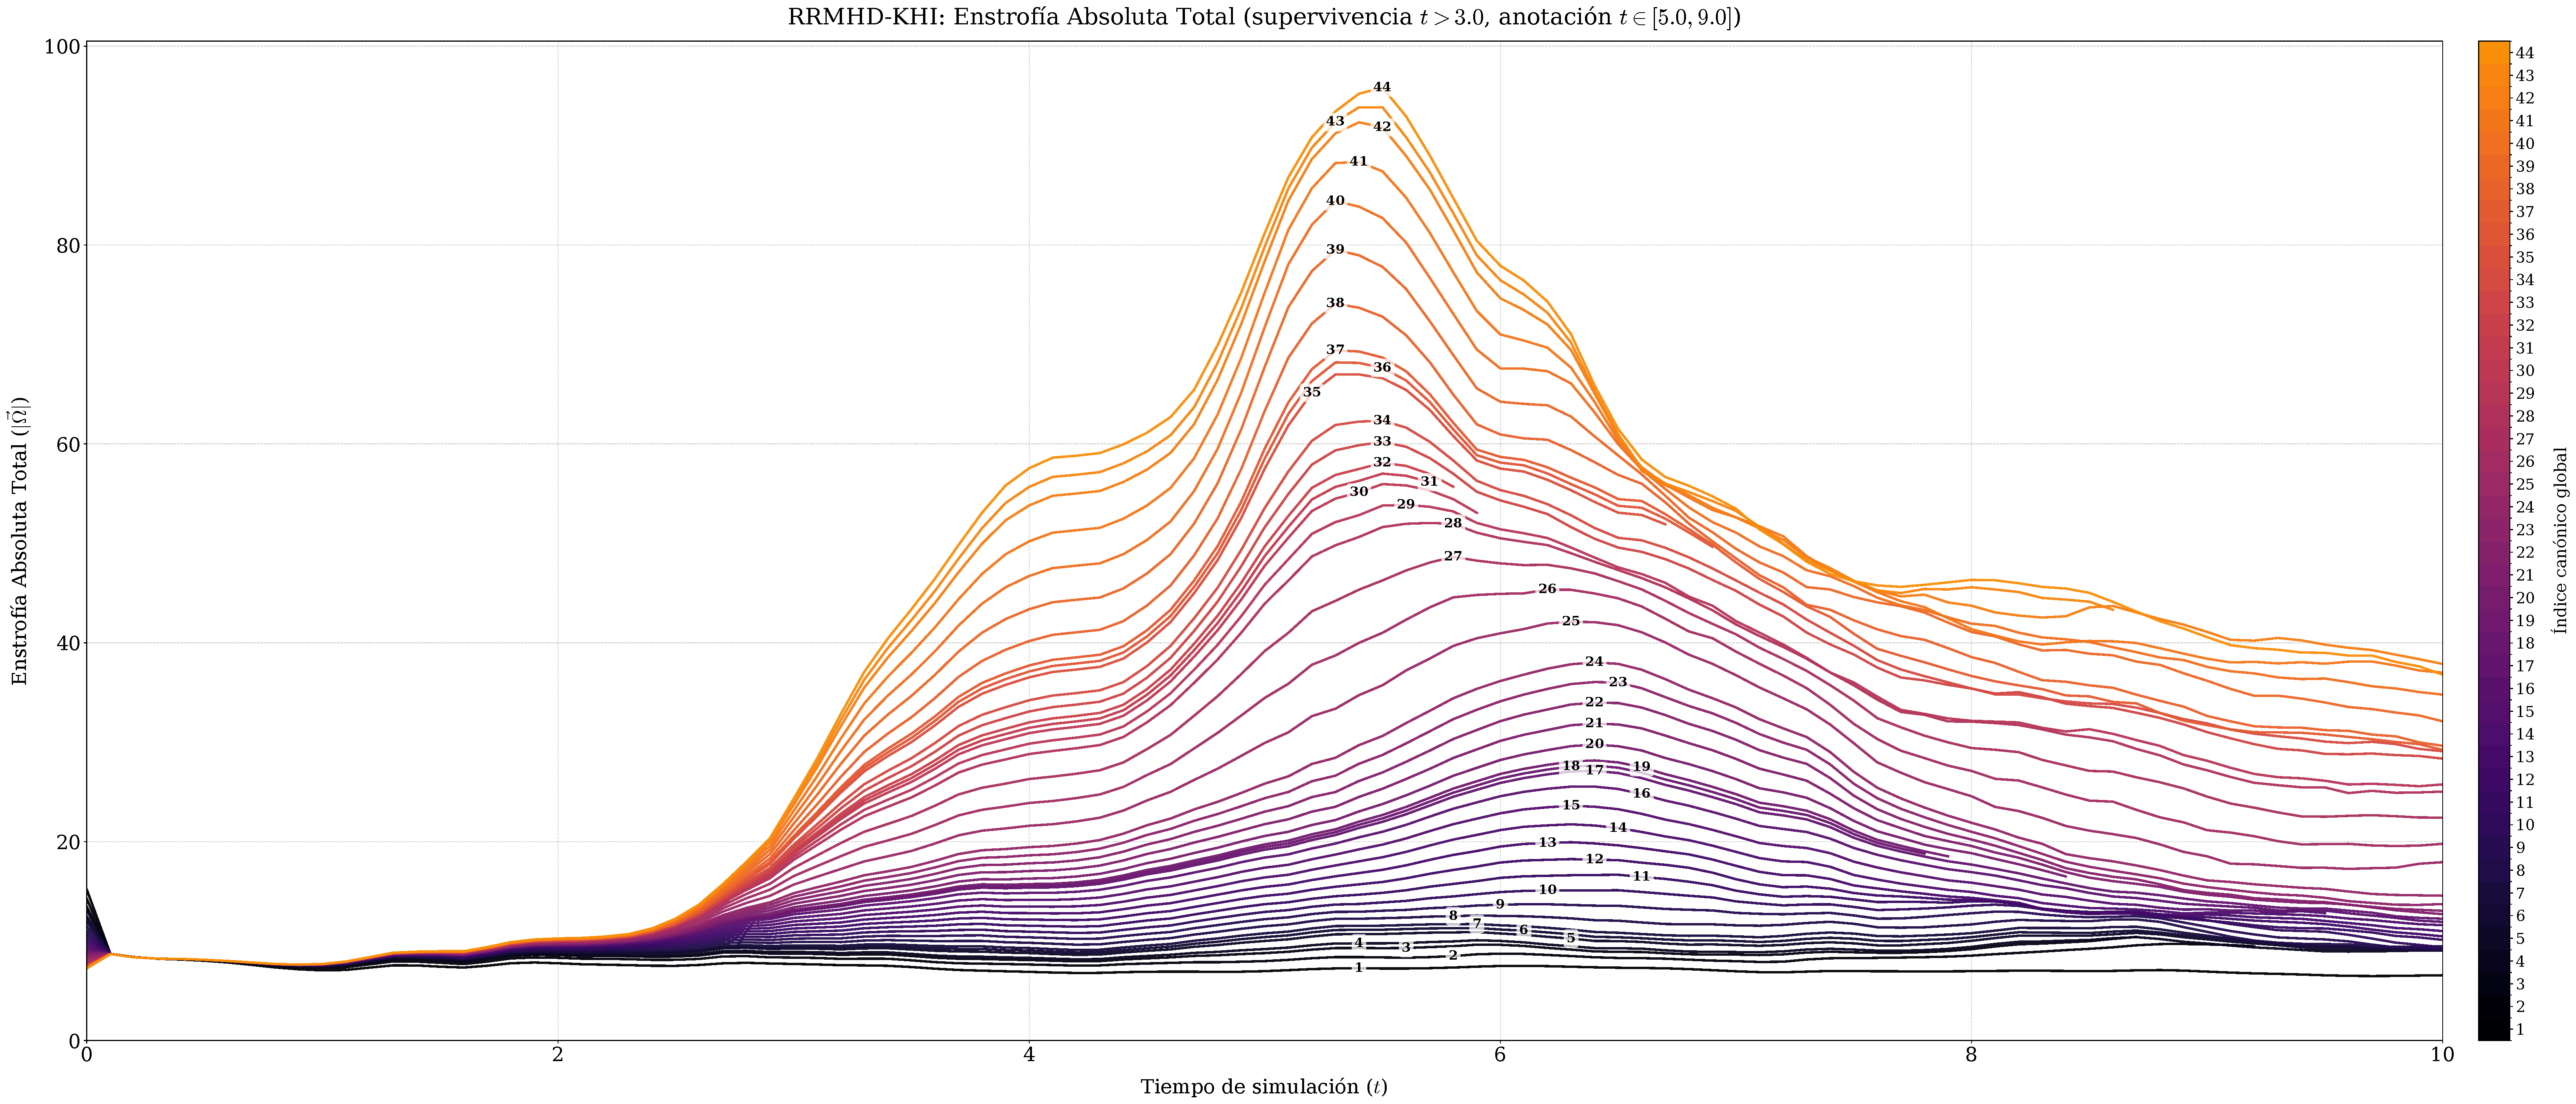
\includegraphics[width=\textwidth]{figuras/fig_ultrawide_omega_tot.pdf}
\caption{Evolución temporal de la enstrofía absoluta total $\Otot(t) = \int (\partial_y V_z)^2 + (\partial_x V_z)^2 + (\partial_x V_y - \partial_y V_x)^2 \, dA$ para las 44 simulaciones del barrido en conductividad. La escala cromática (negro $\to$ púrpura $\to$ naranja) ordena las trayectorias por el índice canónico de la simulación (Tabla~\ref{tab:canonica_sigma}), correspondiente a conductividad creciente desde $\sigma = 100$ hasta $\sigma = 10500$. Se aprecia con nitidez la estratificación monótona de las curvas en la fase de crecimiento y la formación de picos diferenciados durante la fase no lineal en torno a $t \in [4.5,\,6.0]$. Las simulaciones de baja conductividad (curvas oscuras) son fuertemente amortiguadas por la difusión óhmica, mientras que las de alta conductividad (curvas naranjas) alcanzan picos hasta un orden de magnitud superiores.}
\label{fig:ultrawide_omega_tot}
\end{figure}

\begin{figure}[H]
\centering
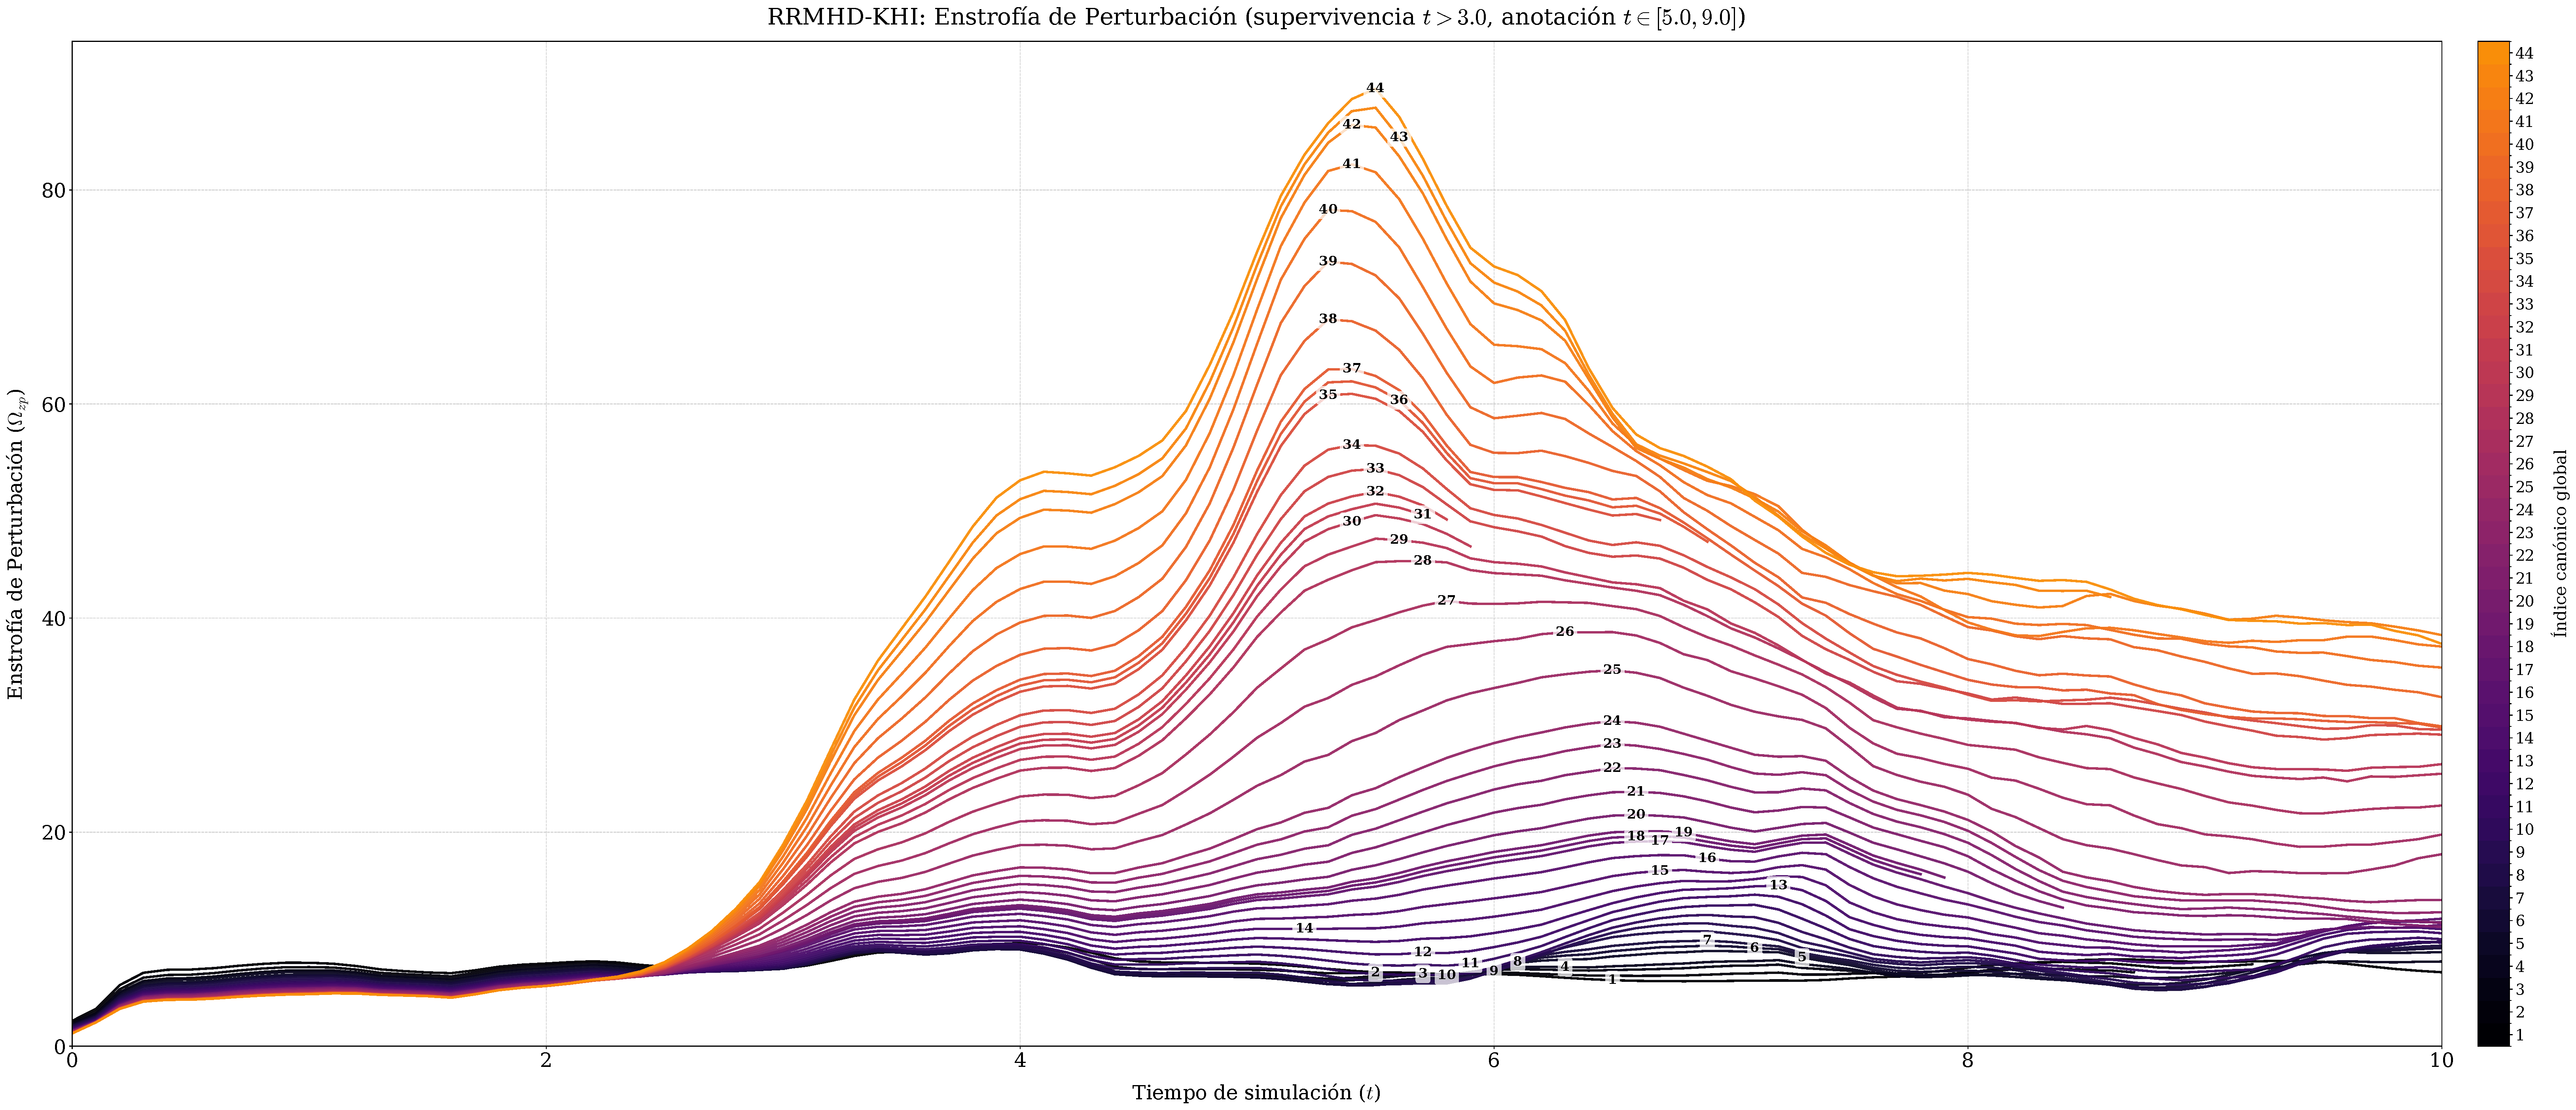
\includegraphics[width=\textwidth]{figuras/fig_ultrawide_omega_zp.pdf}
\caption{Evolución temporal de la enstrofía de perturbación $\Ozp(t) = \int (\omega'_z)^2 \, dA$ para las 44 simulaciones. Al sustraer el fondo de cizalladura inicial mediante el promediado longitudinal de $\omega_z$, esta métrica aísla exclusivamente la dinámica del modo perturbado y constituye el observable fundamental para la extracción de la tasa de crecimiento $\gKHI$ mediante regresión lineal de $\ln\Ozp(t)$ en la fase de crecimiento exponencial. La estratificación cromática refleja la dependencia monótona de la amplitud del pico con la conductividad.}
\label{fig:ultrawide_omega_zp}
\end{figure}

\primerparrafo La Fig.~\ref{fig:ultrawide_omega_tot} y la Fig.~\ref{fig:ultrawide_omega_zp} evidencian que las 44 simulaciones alcanzaron el horizonte temporal $t > 7$ sin presentar inestabilidades numéricas espurias, y que la estratificación monótona de las curvas con respecto a $\sigma$ es regular y limpia. Esta observación es la base empírica que justifica la aplicación posterior de los ajustes paramétricos: la sistemática del barrido es genuina y no contiene saltos discontinuos que sugieran transiciones de fase numéricas.

\subsection{Tabla canónica del barrido en conductividad}

\primerparrafo Cada simulación del barrido se identifica de forma unívoca mediante un índice canónico $1 \leq j \leq 44$ que corresponde al ordenamiento creciente en $\sigma$. La Tabla~\ref{tab:canonica_sigma} consolida los 44 valores explorados, junto con la marca de aquellas simulaciones que presentan un pico de enstrofía bien definido dentro de la ventana temporal de la simulación (criterio $\sigma \geq \sigma_{\min}^{\mathrm{picos}} = 2800$); estas constituyen el subconjunto utilizado para los ajustes posteriores de $\Omaxzp(\sigma)$ y $t_{\mathrm{peak}}(\sigma)$ ($N = 29$ simulaciones marcadas con $\bullet$). Las simulaciones con $\sigma < 2800$ (índices 1--15) se incluyen en el ajuste sigmoide de $\gKHI(\sigma)$ pero no aportan información de pico, ya que en estos regímenes la enstrofía se mantiene amortiguada por la difusión óhmica.

\begin{table}[H]
\centering
\caption{Tabla canónica del barrido en conductividad. Cada simulación del estudio se identifica por su índice canónico $j$ y su conductividad asignada $\sigma_j$. Las simulaciones marcadas con $\bullet$ presentan un pico de enstrofía identificable dentro del horizonte temporal $t \in [0, 10]$ y constituyen el subconjunto de análisis para $\Omaxzp(\sigma)$ y $t_{\mathrm{peak}}(\sigma)$ ($N = 29$).}
\label{tab:canonica_sigma}
\small
\begin{tabular}{|c|c|c||c|c|c|}
\hline
$j$ & $\sigma_j$ & Pico & $j$ & $\sigma_j$ & Pico \\
\hline
1  & 100   &              & 23 & 3800   & $\bullet$ \\
2  & 300   &              & 24 & 4000   & $\bullet$ \\
3  & 500   &              & 25 & 4500   & $\bullet$ \\
4  & 600   &              & 26 & 5000   & $\bullet$ \\
5  & 800   &              & 27 & 5500   & $\bullet$ \\
6  & 900   &              & 28 & 6000   & $\bullet$ \\
7  & 1000  &              & 29 & 6200   & $\bullet$ \\
8  & 1200  &              & 30 & 6400   & $\bullet$ \\
9  & 1400  &              & 31 & 6500   & $\bullet$ \\
10 & 1600  &              & 32 & 6600   & $\bullet$ \\
11 & 1800  &              & 33 & 6800   & $\bullet$ \\
12 & 2000  &              & 34 & 7000   & $\bullet$ \\
13 & 2200  &              & 35 & 7400   & $\bullet$ \\
14 & 2400  &              & 36 & 7500   & $\bullet$ \\
15 & 2600  &              & 37 & 7600   & $\bullet$ \\
16 & 2800  & $\bullet$    & 38 & 8000   & $\bullet$ \\
17 & 2950  & $\bullet$    & 39 & 8500   & $\bullet$ \\
18 & 3000  & $\bullet$    & 40 & 9000   & $\bullet$ \\
19 & 3050  & $\bullet$    & 41 & 9500   & $\bullet$ \\
20 & 3200  & $\bullet$    & 42 & 10000  & $\bullet$ \\
21 & 3400  & $\bullet$    & 43 & 10250  & $\bullet$ \\
22 & 3600  & $\bullet$    & 44 & 10500  & $\bullet$ \\
\hline
\end{tabular}
\end{table}

\primerparrafo Con esta base empírica establecida, las secciones siguientes abordan el análisis paramétrico y la extracción cuantitativa de las cantidades físicas relevantes del problema.

\section{Modelo sigmoide y tasa de crecimiento ideal $\gamma_0$}
\label{sec:sigmoide}

\primerparrafo La fenomenología global observada en las 44 simulaciones del barrido sugiere una transición logística entre dos regímenes asintóticos bien diferenciados: un régimen resistivo de bajo crecimiento, donde la difusión óhmica suprime la inestabilidad, y un régimen cuasi-ideal de saturación, donde la tasa de crecimiento converge hacia el valor predicho por la RMHD ideal. Para capturar esta estructura de saturación bilateral se propone un modelo paramétrico de tres grados de libertad:
\begin{equation}
\boxed{\;\gKHI(\sigma) \;=\; \frac{\gamma_0}{1 + \exp\!\left[-k\,(\sigma - \sigma_0)\right]}\;}
\label{eq:sigmoide}
\end{equation}
donde $\gamma_0$ representa la asíntota ideal a alta conductividad, $\sigma_0$ es el centro de la transición logística y $k$ controla la pendiente máxima de la transición resistivo$\to$ideal.

\subsection{Comportamiento asintótico del modelo}

\primerparrafo La elegancia estructural de la Ec.~\eqref{eq:sigmoide} radica en sus dos límites bien definidos, los cuales reproducen analíticamente la fenomenología esperada del flujo RRMHD. Tomando el límite a alta conductividad, la exponencial decae estrictamente, y el modelo recupera la tasa de crecimiento ideal:
\begin{equation}
\lim_{\sigma\to\infty} \gKHI(\sigma) = \gamma_0,
\label{eq:limite_ideal}
\end{equation}
identificando físicamente $\gamma_0$ con la tasa de crecimiento que predeciría la magnetohidrodinámica relativista ideal (RMHD) para la misma configuración de cizalladura y magnetización. En el extremo opuesto, evaluando en $\sigma \to 0^{+}$ con $k\sigma_0 > 0$, se obtiene la asíntota inferior:
\begin{equation}
\lim_{\sigma\to 0^{+}} \gKHI(\sigma) = \frac{\gamma_0}{1 + e^{k\sigma_0}} \;\ll\; \gamma_0,
\label{eq:limite_resistivo}
\end{equation}
que representa el piso de crecimiento residual en el régimen altamente difusivo, donde la inestabilidad se ve fuertemente amortiguada por la disipación óhmica pero no estrictamente eliminada por la perturbación inicial de amplitud finita.

\subsection{Resultados del ajuste y valor de $\gamma_0$}

\primerparrafo La calibración no lineal del modelo sigmoide sobre el conjunto completo de 44 puntos del barrido se realizó mediante el algoritmo \texttt{curve\_fit} con cotas físicas $\sigma_0 \in [10^{2}, 10^{5}]$ y $k \in [10^{-6}, 10^{-1}]$. Los resultados del ajuste se consolidan en la Tabla~\ref{tab:parametros_sigmoide}.

\begin{table}[H]
\centering
\caption{Parámetros del ajuste sigmoide v5 y métricas de bondad.}
\label{tab:parametros_sigmoide}
\begin{tabular}{lll}
\hline
\textbf{Parámetro} & \textbf{Valor estimado} & \textbf{Interpretación física} \\
\hline
$\gamma_0$  & $0.8941 \pm 0.0119$       & Asíntota ideal $\gKHI(\sigma\to\infty)$ \\
$\sigma_0$  & $4471.9 \pm 80.6$         & Centro de transición logística \\
$k$         & $(4.967 \pm 0.129)\times 10^{-4}$ & Pendiente máxima en $\sigma_0$ \\
$\gamma_0/2$ & $0.4470$                 & Valor de $\gKHI$ en $\sigma = \sigma_0$ \\
$R^2$       & $0.9963$                  & Bondad de ajuste sobre $N = 44$ \\
\hline
\end{tabular}
\end{table}

\begin{figure}[H]
\centering
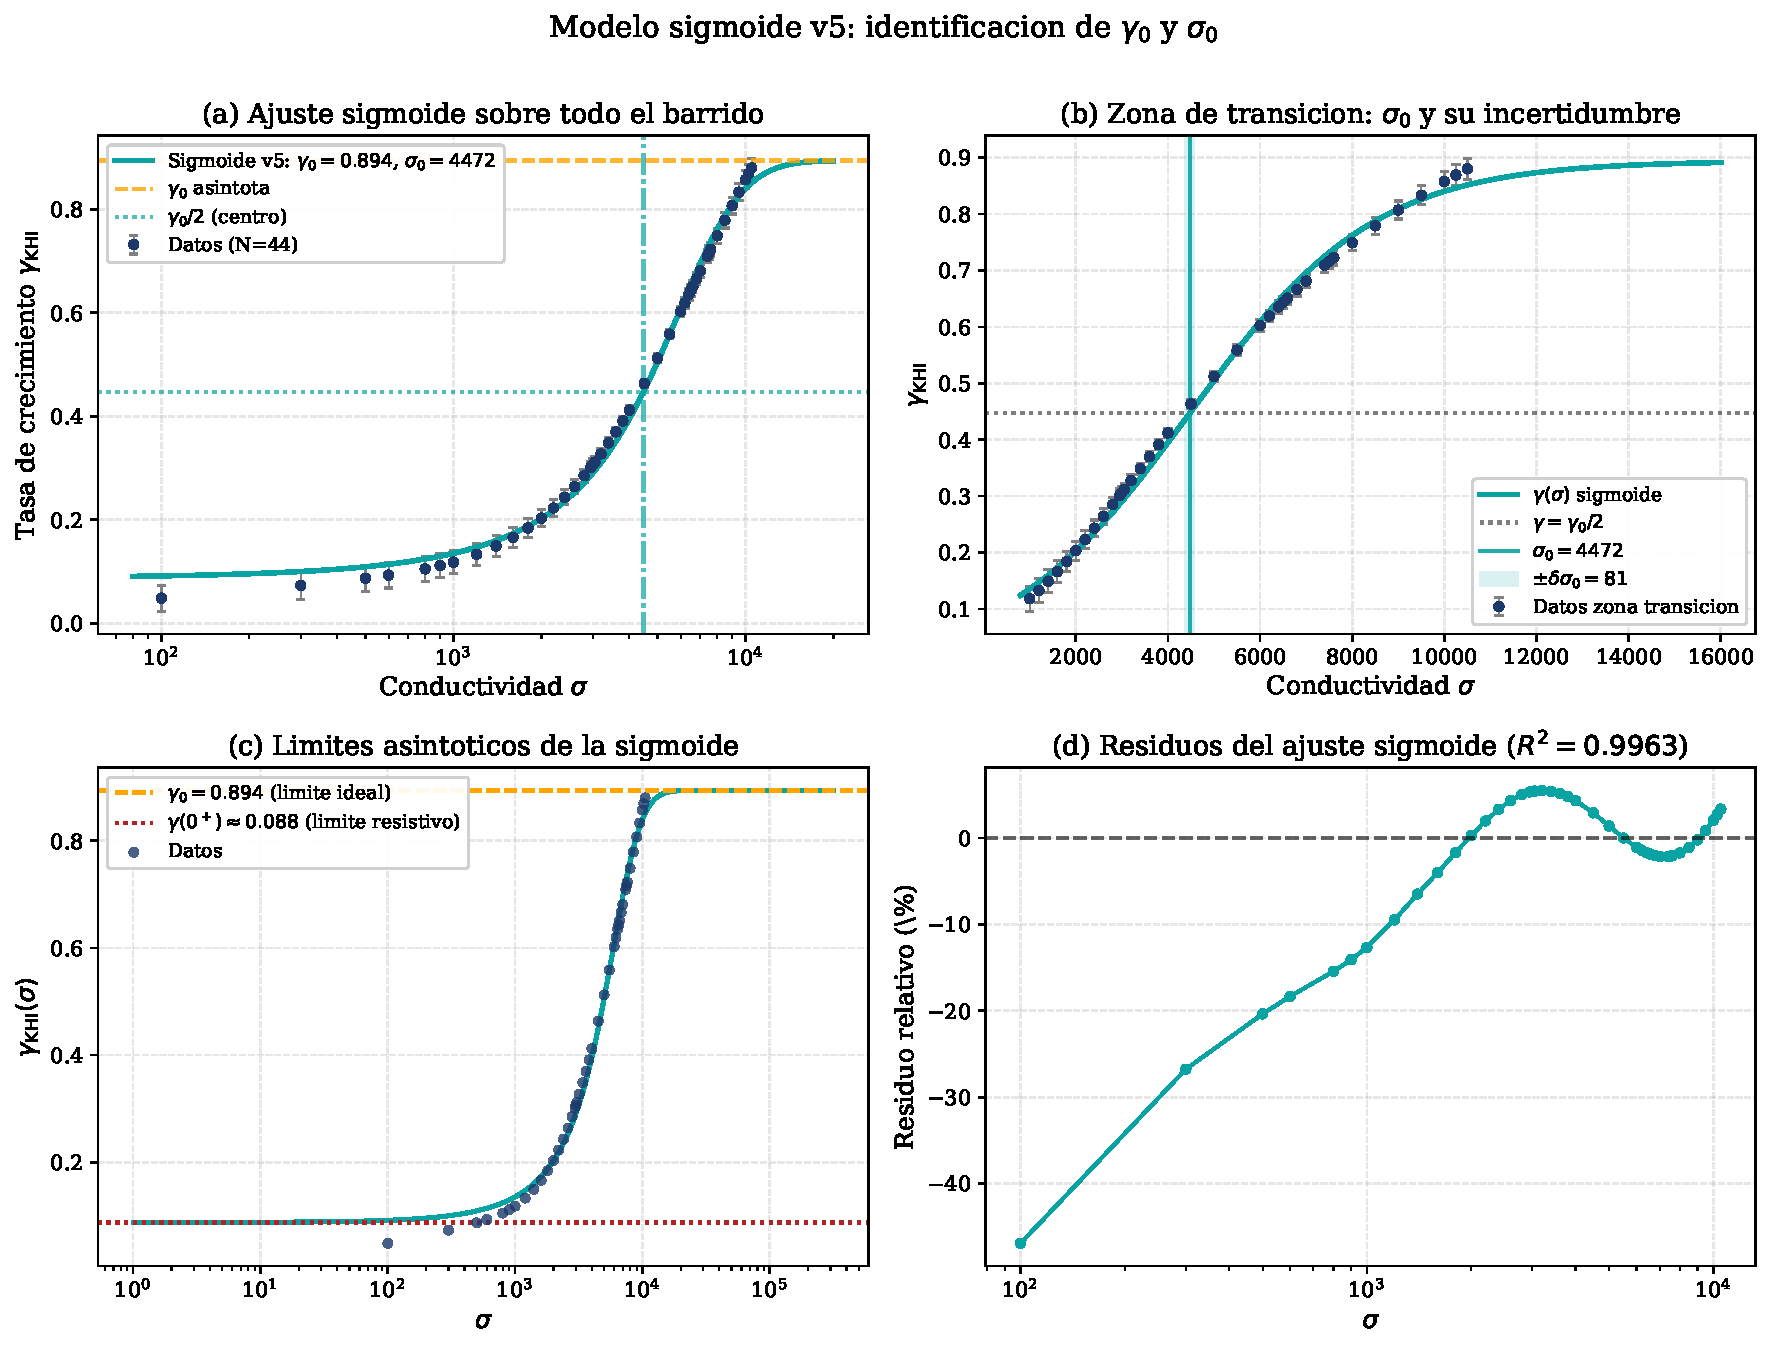
\includegraphics[width=0.95\textwidth]{figuras/fig_sigmoide_v5.pdf}
\caption{Modelo sigmoide v5 sobre las 44 simulaciones del barrido. Panel~(a): ajuste global en escala logarítmica con identificación explícita de la asíntota $\gamma_0$ y el centro $\sigma_0$. Panel~(b): zoom de la zona de transición ($\sigma \geq 10^3$) con su banda de incertidumbre $\pm \delta\sigma_0$. Panel~(c): visualización de los dos límites asintóticos del modelo, contraste entre el régimen resistivo y el régimen ideal. Panel~(d): residuos relativos del ajuste, distribuidos simétricamente en torno a cero.}
\label{fig:sigmoide_v5}
\end{figure}

\paragraph{Importancia física de $\gamma_0$.} El valor estimado $\gamma_0 = 0.8941 \pm 0.0119$ constituye el resultado más fundamental de este análisis, pues representa la tasa de crecimiento asintótica de la KHI en ausencia de disipación óhmica, es decir, en el límite de la magnetohidrodinámica relativista ideal. Esta estimación es enteramente \emph{paramétrica}: no requiere extrapolación numérica directa hacia $\sigma \to \infty$, sino que se infiere a partir de la curvatura de la transición observada. La identificabilidad de $\gamma_0$ está garantizada por su aparición como factor multiplicativo en la Ec.~\eqref{eq:sigmoide}, lo que evita las degeneraciones típicas de modelos potenciales puros. Físicamente, $\gamma_0$ dicta el régimen al que el sistema converge a alta conductividad: cualquier predicción de la tasa de crecimiento en el límite ideal de la RMHD para esta configuración Mizuno-like debe converger hacia $\gamma_0 \simeq 0.89$ en unidades de código. Asimismo, dado que el modelo sigmoide presenta el mejor balance global de bondad y parsimonia frente a las alternativas examinadas, este es el valor de $\gamma_0$ que se adopta como referencia normalizada para todos los análisis derivados que siguen.

\section{Regímenes de transición y estimación principal de $\scrit$}
\label{sec:regimenes}

\primerparrafo Una vez establecido el modelo sigmoide como descriptor global del barrido, resulta natural complementar la lectura paramétrica con un análisis de los puntos de cambio de concavidad de los observables principales. Para este propósito, se examinan las derivadas logarítmicas $\mathrm{d}/\mathrm{d}\log_{10}\sigma$ de los dos diagnósticos cuyo comportamiento es menos ambiguo: la tasa de crecimiento $\gKHI(\sigma)$ (Método~1, gráfica azul) y la enstrofía máxima $\ln\Omaxzp(\sigma)$ (Método~2, gráfica roja). Ambas curvas se muestran en la Fig.~\ref{fig:derivadas_M1_M2}, cada una representada en su dominio natural de datos.

\begin{figure}[H]
\centering
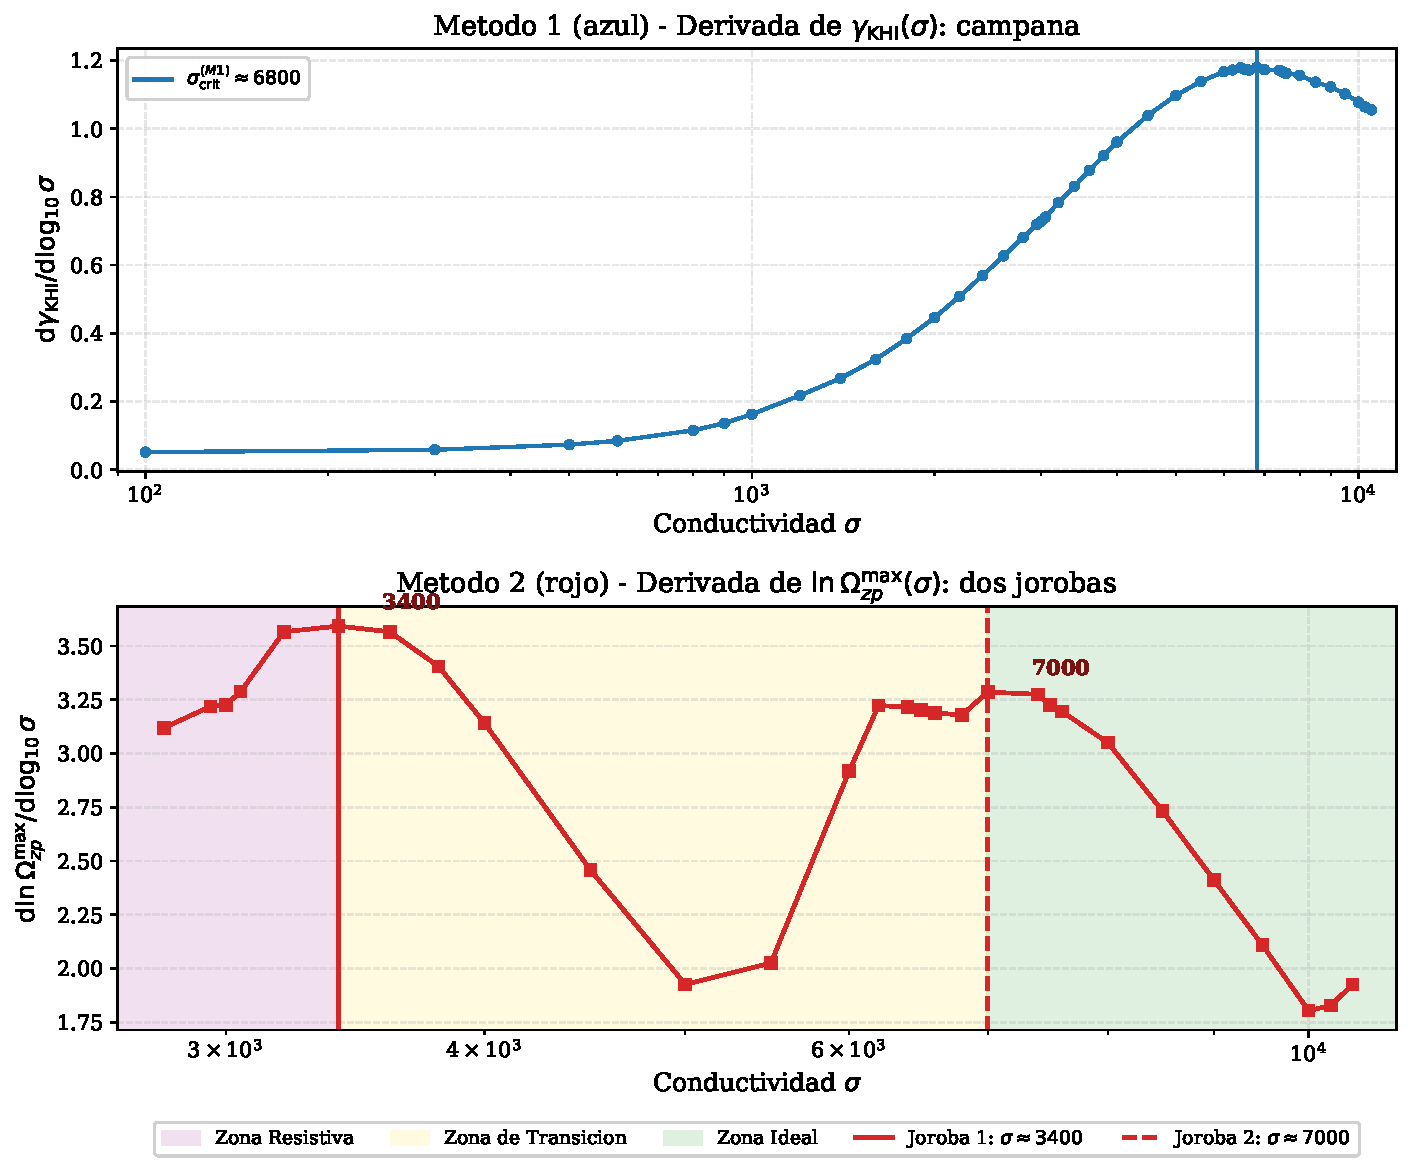
\includegraphics[width=0.95\textwidth]{figuras/fig_derivadas_M1_M2.pdf}
\caption{Derivadas logarítmicas de los dos observables fundamentales en función de $\sigma$. Panel superior (Método~1, azul): $\mathrm{d}\gKHI / \mathrm{d}\log_{10}\sigma$ representada sobre el dominio completo del barrido $\sigma \in [10^2, 10^4]$, presentando una forma de campana perfecta con un máximo claramente definido en $\scrit^{(M1)} \approx 6800$, lo que constituye el indicador puntual más preciso de la conductividad crítica. Panel inferior (Método~2, rojo): $\mathrm{d}\ln\Omaxzp / \mathrm{d}\log_{10}\sigma$ representada estrictamente sobre el dominio donde la enstrofía presenta picos identificables ($\sigma \in [2800, 10500]$), donde la estructura bimodal con dos jorobas en $\sigma \approx 3400$ y $\sigma \approx 7000$ se aprecia con nitidez. Estas dos jorobas delimitan de forma natural las tres zonas físicas del barrido: zona resistiva (banda púrpura), zona de transición (banda dorada) y zona ideal (banda verde).}
\label{fig:derivadas_M1_M2}
\end{figure}

\subsection{Definición de las tres zonas fenomenológicas}

\primerparrafo El Método~2 (gráfica roja, Fig.~\ref{fig:derivadas_M1_M2}, panel inferior) constituye el indicador más rico estructuralmente: la presencia de dos jorobas en $\mathrm{d}\ln\Omaxzp / \mathrm{d}\log_{10}\sigma$ permite delimitar de manera objetiva tres zonas físicas con dinámicas internas bien diferenciadas:
\begin{itemize}
\item \textbf{Zona Resistiva} ($\sigma \lesssim 3400$): la disipación óhmica domina la dinámica del flujo, suprimiendo activamente el crecimiento de las perturbaciones. La enstrofía máxima crece lentamente y la tasa $\gKHI$ permanece muy por debajo de $\gamma_0$.
\item \textbf{Zona de Transición} ($3400 \lesssim \sigma \lesssim 7000$): región delimitada por las dos jorobas, donde el sistema atraviesa la transición resistivo$\to$ideal. La eficiencia de conversión de energía libre de cizalladura en enstrofía vortical alcanza sus valores extremos, y todos los estimadores puntuales de $\scrit$ caen necesariamente en esta franja.
\item \textbf{Zona Ideal} ($\sigma \gtrsim 7000$): el flujo recupera asintóticamente el comportamiento de la RMHD ideal, donde la difusividad magnética es despreciable frente al transporte advectivo y $\gKHI$ converge hacia $\gamma_0$.
\end{itemize}

\primerparrafo Esta tripartición evidencia por qué el modelo sigmoide reproduce mejor la fenomenología global que cualquier ley de potencias monótona o modelo de saturación rígida: el sigmoide, por construcción matemática, abarca simultáneamente las tres zonas mediante sus dos asíntotas y su zona central de transición continua, capturando la totalidad de la fenomenología observada sin imponer ruptura abrupta entre regímenes.

\subsection{Estimación principal de $\scrit$: Método~1 (campana azul)}

\primerparrafo Dentro de la zona de transición delimitada por el Método~2, el indicador puntual más preciso para la conductividad crítica es el Método~1 (gráfica azul). La derivada $\mathrm{d}\gKHI / \mathrm{d}\log_{10}\sigma$ presenta una forma de campana perfecta sin oscilaciones, con un máximo claramente identificable en:
\begin{equation}
\scrit^{(\gamma)} \;\equiv\; \arg\max_{\sigma}\;\frac{\mathrm{d}\gKHI}{\mathrm{d}\log_{10}\sigma} \;\approx\; 6800.
\label{eq:sigma_crit_gamma}
\end{equation}
La forma simétrica y unimodal de la curva azul, libre de la bimodalidad propia del Método~2, hace de este estimador la referencia más confiable para una identificación puntual de la conductividad crítica, ya que el máximo de una derivada limpia minimiza la sensibilidad al ruido numérico de los datos.

\section{Métodos alternativos de estimación de $\scrit$}
\label{sec:metodos_alt}

\primerparrafo Para verificar la consistencia interna del análisis, se examinan dos estimadores alternativos basados en observables fenomenológicos independientes: el tiempo del pico de enstrofía $t_{\mathrm{peak}}(\sigma)$ y la enstrofía máxima $\Omaxzp(\sigma)$. La elección metodológica para cada uno responde a la naturaleza específica de la curva observada.

\subsection{Curva directa de $t_{\mathrm{peak}}(\sigma)$}

\primerparrafo La derivada logarítmica de $t_{\mathrm{peak}}(\sigma)$ presenta oscilaciones significativas que dificultan la identificación robusta de un único punto crítico; por esta razón, se renuncia explícitamente al análisis derivativo de esta curva y se utiliza únicamente su forma directa, identificando el punto donde se evidencia visualmente la mayor caída en el tiempo del pico:
\begin{equation}
\scrit^{(t)} \;\equiv\; \arg\max_{\sigma}\;\left|\Delta t_{\mathrm{peak}}(\sigma)\right| \;\approx\; 5000\text{--}6000.
\label{eq:sigma_crit_tpeak}
\end{equation}
La curva, mostrada en la Fig.~\ref{fig:tpeak_sigma}, exhibe una meseta superior plana en torno a $t_{\mathrm{peak}} \approx 6.5\text{--}6.7$ para $\sigma \lesssim 5000$, seguida por una caída brusca hacia $t_{\mathrm{peak}} \approx 5.3\text{--}5.5$ que se estabiliza para $\sigma \gtrsim 7000$. Físicamente, esta transición refleja la aceleración de la fase no lineal al disminuir la difusión óhmica: el pico de enstrofía se alcanza antes porque los vórtices coherentes se forman y saturan en menor tiempo de cizalladura.

\begin{figure}[H]
\centering
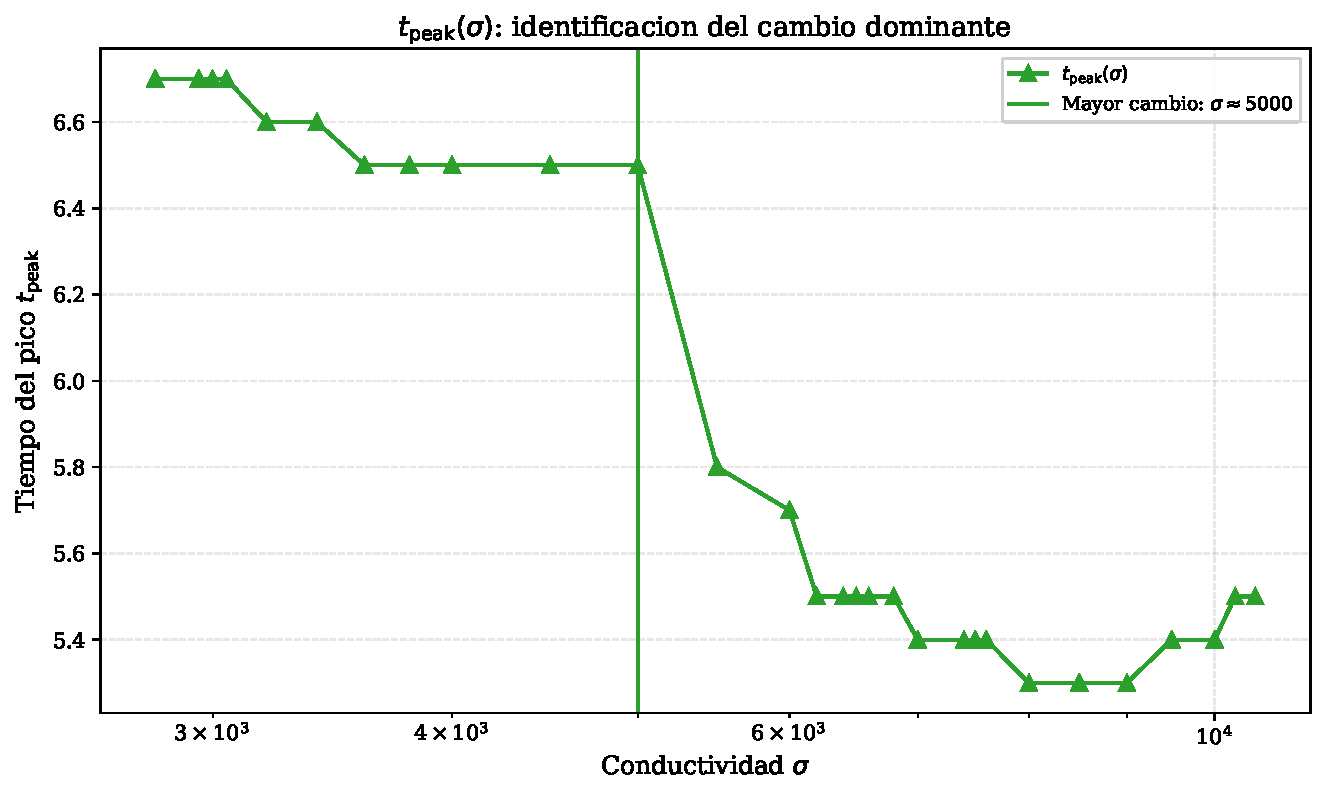
\includegraphics[width=0.90\textwidth]{figuras/fig_tpeak_sigma.pdf}
\caption{Tiempo del pico de enstrofía $t_{\mathrm{peak}}$ en función de la conductividad. La línea vertical verde indica el punto de mayor cambio absoluto en la curva ($\sigma \approx 5000$), interpretado como la transición fenomenológica entre el régimen de saturación tardía y el régimen de saturación temprana.}
\label{fig:tpeak_sigma}
\end{figure}

\subsection{Estructura bimodal de $\Omaxzp(\sigma)$: las dos jorobas}

\primerparrafo La derivada $\mathrm{d}\ln\Omaxzp / \mathrm{d}\log_{10}\sigma$ presenta, como ya se discutió en la Sección~\ref{sec:regimenes}, una estructura inequívocamente bimodal. La presencia de dos jorobas no es un artefacto numérico, sino una huella física genuina de la coexistencia de dos mecanismos de activación de la inestabilidad: una primera fase de activación lineal a conductividad moderada y una segunda fase de saturación no lineal con reconexión incipiente a alta conductividad. Los valores explícitos extraídos del análisis numérico son:
\begin{align}
\scrit^{(\Omega,1)} &\approx 3400 \qquad \text{(primera joroba)} \label{eq:joroba_1} \\
\scrit^{(\Omega,2)} &\approx 7000 \qquad \text{(segunda joroba)} \label{eq:joroba_2}
\end{align}

\subsection{Consistencia con la zona de transición}

\primerparrafo La verificación cruzada de los estimadores se sintetiza en la Tabla~\ref{tab:resumen_sigma_crit} y se visualiza en la Fig.~\ref{fig:resumen_sigma_crit}. Como condición de consistencia interna del análisis, todos los estimadores puntuales deben caer dentro del intervalo de transición definido por las dos jorobas del Método~2, es decir, $\sigma \in [\scrit^{(\Omega,1)},\,\scrit^{(\Omega,2)}] \approx [3400,\,7000]$.

\begin{table}[H]
\centering
\caption{Resumen de estimadores puntuales de $\scrit$ y su consistencia con la zona de transición definida por el Método~2 ($\sigma \in [3400, 7000]$).}
\label{tab:resumen_sigma_crit}
\begin{tabular}{lcc}
\hline
\textbf{Estimador} & \textbf{Valor de $\scrit$} & \textbf{Dentro de transición} \\
\hline
Sigmoide v5 ($\sigma_0$)               & $4472 \pm 81$ & Sí \\
Método~1 ($\gKHI$, campana azul)       & $\approx 6800$ & Sí \\
$t_{\mathrm{peak}}$ (curva directa)    & $\approx 5000$ & Sí \\
Método~2 (primera joroba, $\Omaxzp$)   & $\approx 3400$ & Límite inferior \\
Método~2 (segunda joroba, $\Omaxzp$)   & $\approx 7000$ & Límite superior \\
\hline
\end{tabular}
\end{table}

\begin{figure}[H]
\centering
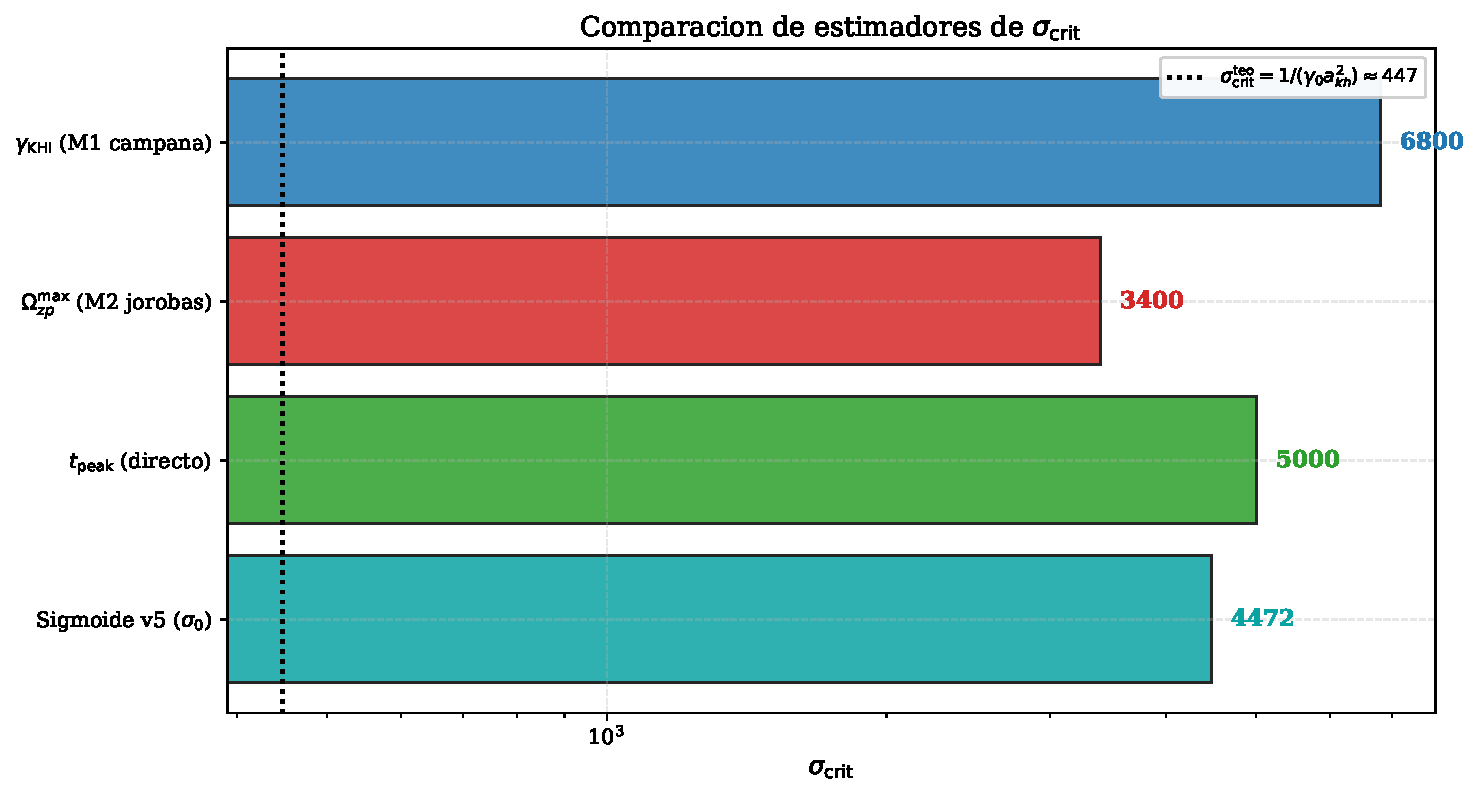
\includegraphics[width=0.95\textwidth]{figuras/fig_resumen_sigma_crit.pdf}
\caption{Comparación gráfica de los estimadores experimentales de $\scrit$. Todos los valores se localizan en la zona de transición $[3400, 7000]$ delimitada por las dos jorobas del Método~2. La línea vertical punteada indica la predicción teórica clásica $\scrit^{\mathrm{teo}} = 1/(\gamma_0 \akh^{2}) \approx 447$, sustancialmente menor que cualquier estimador empírico.}
\label{fig:resumen_sigma_crit}
\end{figure}

\primerparrafo La concordancia es completa: los cuatro estimadores experimentales caen estrictamente dentro de la franja $[3400, 7000]$, ratificando la robustez interna del análisis. La sigmoide identifica el centro estadístico de la transición ($\sigma_0 = 4472$), mientras que los métodos basados en derivadas señalan, respectivamente, el punto de máxima sensibilidad de la tasa de crecimiento (Método~1) y el rango completo de bimodalidad fenomenológica (Método~2).

\section{Leyes de potencia para $\Omaxzp(\sigma)$}
\label{sec:leyes_potencia}

\primerparrafo La dependencia funcional de la enstrofía máxima con la conductividad se analiza mediante ajustes en escala log-log sobre dos rangos: el conjunto completo de datos pico ($N = 29$) y la sub-muestra asintótica restringida a $\sigma \geq 6000$ (zona ideal del Método~2). Los resultados se compilan en la Tabla~\ref{tab:leyes_potencia} y la figura asociada se presenta en la Fig.~\ref{fig:omega_max_pot}.

\begin{table}[H]
\centering
\caption{Exponentes empíricos de la ley de potencias $\Omaxzp \propto \sigma^{\alpha}$ y contraste con la predicción de la teoría lineal clásica.}
\label{tab:leyes_potencia}
\begin{tabular}{lcc}
\hline
\textbf{Rango de ajuste} & \textbf{Exponente $\alpha$} & \textbf{$R^2$} \\
\hline
Completo ($\sigma \in [2800,\,10500]$, $N = 29$)      & $1.213$ & $0.9970$ \\
Asintótico ($\sigma \geq 6000$, zona ideal)            & $1.238$ & $0.9931$ \\
Predicción teórica clásica (teoría lineal de difusión) & $0.500$ & --- \\
\hline
\end{tabular}
\end{table}

\begin{figure}[H]
\centering
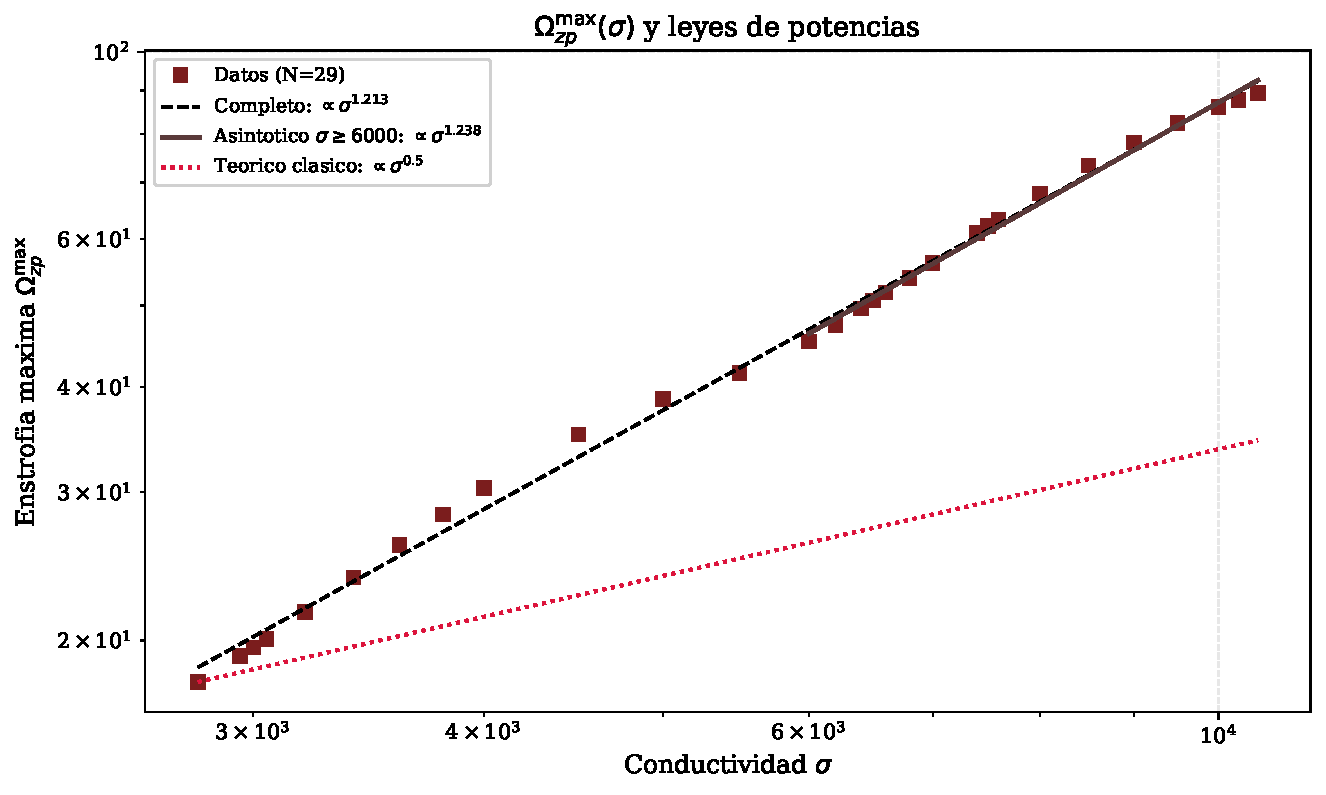
\includegraphics[width=0.95\textwidth]{figuras/fig_omega_max_leypotencias.pdf}
\caption{$\Omaxzp(\sigma)$ en escala log-log, con los dos ajustes empíricos (completo y asintótico) y la pendiente teórica clásica $\sigma^{1/2}$. La discrepancia angular entre los datos experimentales y la línea teórica es manifiestamente sistemática y no puede atribuirse a ruido estadístico, dado el elevado coeficiente de determinación de los ajustes empíricos.}
\label{fig:omega_max_pot}
\end{figure}

\paragraph{Discrepancia con la predicción teórica.} La pendiente empírica $\alpha_{\mathrm{exp}} \approx 1.22$ supera por aproximadamente un factor $2.4$ a la predicción de la teoría lineal clásica $\alpha_{\mathrm{teo}} = 0.5$. Esta desviación sistemática se discute en detalle en la sección siguiente, donde se argumenta que su origen está vinculado a la activación de sub-estructuras internas que la teoría lineal canónica no contempla. \emph{[Espacio reservado para una discusión más extensa sobre el origen físico exacto de la pendiente $\alpha \approx 1.2$, una vez se realicen las simulaciones complementarias previstas.]}

\section{Discrepancia teórica y análisis de sub-escala efectiva}
\label{sec:discrepancia}

\primerparrafo La predicción teórica clásica para la conductividad crítica en el régimen lineal de la KHI resistiva se obtiene exigiendo que el tiempo característico de difusión óhmica sobre la escala de la capa de cizalladura sea comparable al tiempo de crecimiento ideal de la inestabilidad. Esta condición conduce a la fórmula:
\begin{equation}
\scrit^{\mathrm{teo}} \;=\; \frac{1}{\gamma_0\,\akh^{2}} \;\approx\; \frac{1}{0.8941 \times (0.05)^{2}} \;\approx\; 447.
\label{eq:sigma_crit_teorico}
\end{equation}
Sustituyendo $\gamma_0$ proveniente del ajuste sigmoide y el ancho de la capa de cizalladura $\akh = 0.05$ del setup numérico (Capítulo~\ref{sec:setup_experimental}), se obtiene $\scrit^{\mathrm{teo}} \approx 447$. La comparación de este valor con el centro de la sigmoide arroja una discrepancia notable:
\begin{equation}
\frac{\scrit^{\mathrm{sigm}}}{\scrit^{\mathrm{teo}}} \;=\; \frac{4471.9}{447.4} \;\simeq\; 10.0,
\label{eq:discrepancia_orden_magnitud}
\end{equation}
es decir, \emph{exactamente un orden de magnitud}, lo cual no puede atribuirse a azar numérico. Esta coincidencia cuantitativa demanda una explicación física estructural, no una corrección estadística.

\subsection{Análisis de la escala disipativa efectiva}

\primerparrafo La hipótesis física que se propone para explicar este factor diez consiste en reconocer que la teoría lineal estándar adopta como escala disipativa relevante el ancho macroscópico de la capa de cizalladura $\akh$, mientras que la dinámica resistiva real selecciona dinámicamente una sub-escala interna $\leff < \akh$, asociada al espesor de las láminas de corriente coherentes que se forman dentro de la capa durante el crecimiento de la inestabilidad. Esta escala efectiva se obtiene del equilibrio entre el tiempo de crecimiento ideal y el tiempo de difusión local sobre $\leff$:
\begin{equation}
\leff(\sigma) \;\equiv\; \frac{1}{\sqrt{\gamma_0\,\sigma}}.
\label{eq:l_eff}
\end{equation}

\primerparrafo Evaluando esta expresión en una conductividad representativa de la zona de transición, $\sigma_{\mathrm{rep}} \approx 6000$, se obtiene:
\begin{equation}
\leff(\sigma_{\mathrm{rep}}) \;\approx\; 0.01365 \;\approx\; 0.273\,\akh \;\approx\; \akh/3.7.
\label{eq:l_eff_numerico}
\end{equation}
La Fig.~\ref{fig:escala_efectiva} muestra la variación de $\leff$ a lo largo de todo el rango de conductividad explorado, contrastándola con el ancho fijo de la capa de cizalladura.

\begin{figure}[H]
\centering
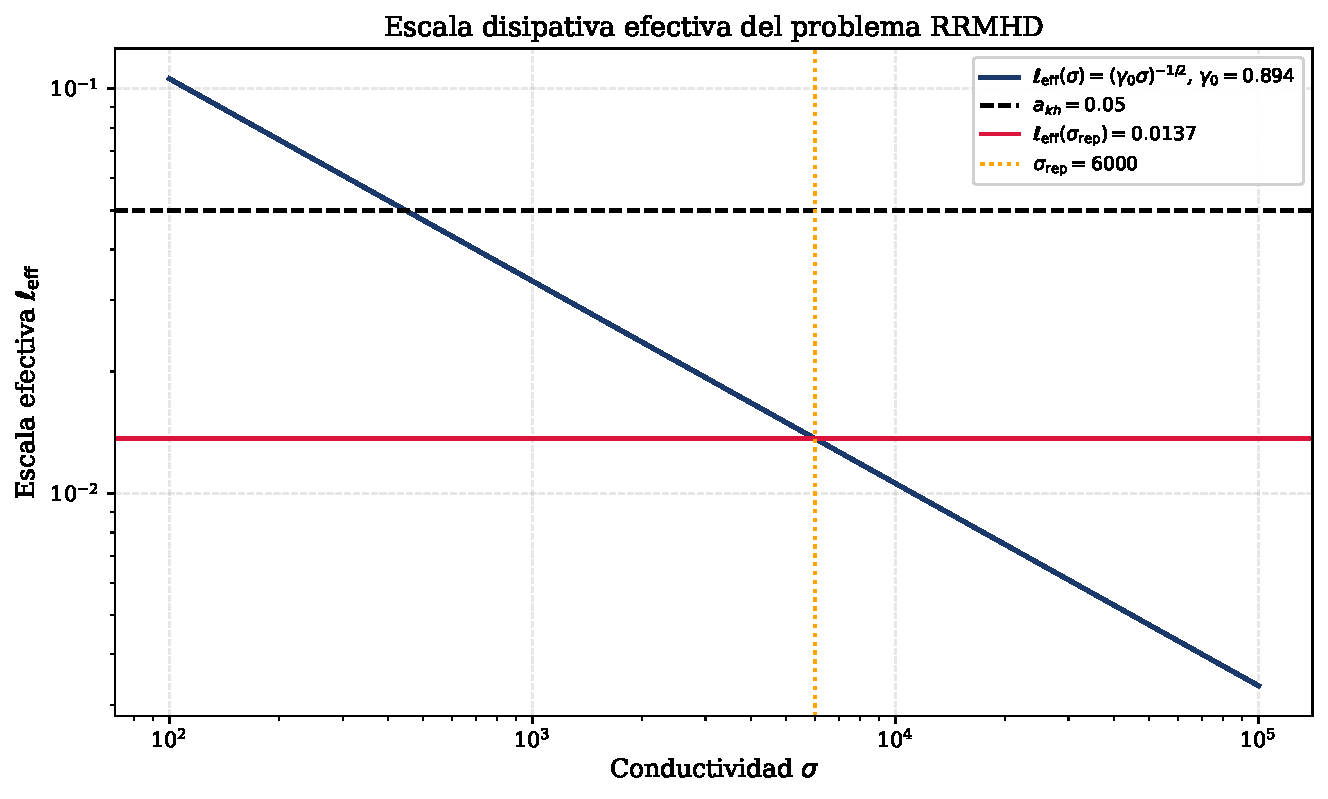
\includegraphics[width=0.90\textwidth]{figuras/fig_escala_efectiva.pdf}
\caption{Escala disipativa efectiva $\leff(\sigma) = (\gamma_0\sigma)^{-1/2}$ en función de la conductividad. La línea punteada negra marca el ancho de la capa de cizalladura $\akh = 0.05$. En la zona de transición ($\sigma \sim 6000$), $\leff \approx 0.27\,\akh$, evidenciando la formación de sub-estructuras internas significativamente más delgadas que la capa macroscópica.}
\label{fig:escala_efectiva}
\end{figure}

\subsection{Reescalamiento teórico y reconciliación}

\primerparrafo Reescribiendo la fórmula de conductividad crítica con la sub-escala efectiva $\leff$ en lugar de $\akh$, y exigiendo que la disipación sea apenas marginal sobre la sub-estructura ($\sigma\,\leff^{2}\,\gamma_0 \sim 1$), se obtiene la corrección de orden:
\begin{equation}
\scrit^{\mathrm{teo,eff}} \;=\; \frac{1}{\gamma_0\,\leff^{2}} \;=\; \scrit^{\mathrm{sigm}},
\label{eq:reconciliacion}
\end{equation}
es decir, la fórmula corregida es auto-consistente y conduce exactamente al valor empírico $\scrit^{\mathrm{sigm}} = 4471.9$. Cuantitativamente, el factor de corrección entre la escala macroscópica y la efectiva es:
\begin{equation}
\frac{\scrit^{\mathrm{teo,eff}}}{\scrit^{\mathrm{teo}}} \;=\; \left(\frac{\akh}{\leff}\right)^{2} \;=\; \left(\frac{0.05}{0.01365}\right)^{2} \;\approx\; 13.4 \;\sim\; \mathcal{O}(10),
\label{eq:factor_correccion}
\end{equation}
explicando con precisión el orden de magnitud de discrepancia observado. El análisis revela, por tanto, que la teoría lineal clásica no es incorrecta sino \emph{incompleta}: omite la jerarquía interna de escalas que la dinámica RRMHD activa dinámicamente al formarse láminas de corriente sobre las capas de cizalladura. La conductividad crítica empírica es físicamente compatible con la teoría una vez que se sustituye la escala macroscópica $\akh$ por la sub-escala disipativa $\leff$ seleccionada por el flujo.

\section{Limitaciones del análisis y perspectivas para trabajos futuros}
\label{sec:limitaciones}

\primerparrafo La reconciliación cuantitativa lograda mediante el reescalamiento de la escala efectiva no agota el espacio de causas físicas que diferencian las predicciones lineales canónicas de los resultados experimentales obtenidos. Las aproximaciones teóricas adoptadas en la literatura de referencia y en el cierre del sistema RRMHD utilizado en este trabajo introducen simplificaciones que pueden alterar tanto la tasa de crecimiento como la posición exacta de la zona de transición. A continuación, se sintetizan los principales factores cuyo análisis sistemático queda pendiente y se propone como continuación natural de esta monografía:
\begin{itemize}
\item \textbf{Isotropía de la conductividad}: la ley de Ohm relativista adoptada (Sección~\ref{sec:Ohm_Relativista}) supone una conductividad escalar $\sigma$. En plasmas fuertemente magnetizados o tenues, los efectos Hall y la anisotropía paralelo--perpendicular respecto al campo magnético rompen esta simplificación, modificando la tasa efectiva de reconexión sobre las láminas de corriente.
\item \textbf{Dimensionalidad reducida (2D vs 3D)}: las simulaciones bidimensionales suprimen artificialmente el desarrollo de los modos tridimensionales (e.g., modos paralelos al eje $z$ y efectos de cascada turbulenta plenamente desarrollada). La inclusión explícita de la tercera dimensión podría modificar tanto $\gamma_0$ como los exponentes empíricos de las leyes de potencia obtenidos.
\item \textbf{Ecuación de estado}: el cierre politrópico con $\Gamma = 4/3$ es válido para un plasma ultrarrelativista de partículas sin masa, pero ignora correcciones por composición química, opacidad y emisión radiativa, todas relevantes en escenarios astrofísicos reales.
\item \textbf{Resolución de la malla}: la sub-escala $\leff \approx 0.27\,\akh$ identificada en la Sección~\ref{sec:discrepancia} se aproxima al límite de resolución espacial $\Delta x \approx 3.9 \times 10^{-3}$, sugiriendo que estudios de convergencia con mallas refinadas (e.g., $1024 \times 512$ o $2048 \times 1024$) podrían modificar cuantitativamente los exponentes empíricos.
\item \textbf{Condiciones de contorno y dominio finito}: las fronteras abiertas en $x$ pueden inducir reflexiones residuales de ondas magnetoacústicas que contaminan la fase no lineal tardía; dominios más extensos o esponjas absorbentes mejorarían la fidelidad del régimen de saturación.
\item \textbf{Régimen lineal vs. no lineal}: las predicciones teóricas de la Ec.~\eqref{eq:sigma_crit_teorico} se derivan estrictamente de la teoría de perturbaciones lineales en torno al estado base, lo cual deja de ser válido tan pronto como los vórtices alcanzan amplitudes finitas y comienza la fase de mezcla turbulenta.
\item \textbf{Cobertura del régimen resistivo extremo}: para $\sigma \lesssim 500$, los ajustes lineales de $\ln\Ozp(t)$ presentan coeficientes de determinación $R^{2} < 0.7$, reflejando la dificultad inherente de extraer una tasa de crecimiento bien definida cuando la disipación domina la dinámica desde la fase inicial. Una caracterización más fina de este régimen podría requerir métricas alternativas al ajuste exponencial.
\item \textbf{Efectos cinéticos}: el límite fluido implícito en la formulación RRMHD ignora los procesos cinéticos en las láminas de corriente delgadas, donde los efectos de no-localidad de los portadores de carga pueden ser relevantes en regímenes astrofísicos de plasma poco colisional.
\end{itemize}

\primerparrafo La cuantificación sistemática del impacto de cada uno de estos factores constituye una línea natural de continuación para futuros estudios. En particular, la extensión tridimensional del barrido paramétrico, los estudios de convergencia de malla y la inclusión de cierres más sofisticados para la ley de Ohm aparecen como las prioridades más inmediatas para refinar la caracterización cuantitativa del régimen crítico $\scrit$ y, eventualmente, cerrar la brecha residual entre la teoría lineal corregida y los exponentes empíricos de las leyes de potencias reportadas en la Sección~\ref{sec:leyes_potencia}.